\documentclass[11pt,a4paper]{article}
\usepackage[utf8]{inputenc}
\usepackage[T1]{fontenc}
% \usepackage{gentium}
\usepackage{mathptmx} % Use Times Font

\usepackage{graphicx} % Required for including pictures
\usepackage{hyperref} % Format links for pdf
\usepackage{biblatex}
\addbibresource{references.bib}
\usepackage{booktabs} % Used so that tables generated by pandas
                      % to_latex() work correctly

\frenchspacing % No double spacing between sentences
\usepackage[margin=1in]{geometry}
% \usepackage[all]{nowidow} % Tries to remove widows
\usepackage[protrusion=true,expansion=true]{microtype} % Improves typography, load after fontpackage is selected


\title{My datascience project title}
\author{Irma Student and Soham Eye}

\begin{document}

\maketitle

%% INSTRUCTIONS:
%%
%% 1. Create your own copy of this Overleaf project. You can either edit your report
%% using:
%%
%%    a. Overleaf professional, a collaborative LaTeX editor. You can click
%%       "Copy Project" from the Overleaf menu to create a version where you have
%%       read and write permissions. See the following for documentation:
%%       https://www.overleaf.com/edu/edinburgh and
%%       https://uoe.sharepoint.com/:f:/r/sites/digitalskillsandtraining/Shared%20Documents/LaTeX/LaTeX%20for%20Beginners%20using%20Overleaf?csf=1&web=1&e=cPqTI3
%%
%%    b. A LaTeX editor on your PC. For this option, you can download the source
%%       of this project as a zip (via the Overleaf menu).
%% 
%% 2. Please rename this file fds-project-option-1.tex, 
%% fds-project-option-2.tex, or fds-project-option-3.tex, depending on
%% which project option you are doing. When you submit, please submit
%% the PDF file with the corresponding name.
%% 
%% 3. Please keep the section and paragraph headings as they
%%    are. You should delete all the text within the headings, e.g.
%%    the text that says "What is the area of this data science
%%    study, and why is it interesting to investigate" and the
%%    bullet points. Keeping the headings makes the report a lot
%%    easier for the markers to read, and making things easy for
%%    markers is always beneficial.
%%
%% 4. The word limit for the Overview section is mandatory. For the
%% other sections word limits are suggested.
%%
%% 5. The page limits must be strictly adhered to, and depend on if
%% you are working individually, in pairs or in threes:
%%
%%   - Individual: 6 pages 
%%   - Pairs: 8 pages 
%%   - Threes: 10 pages 
%%

\section{Overview}
% 250 words maximum

\section{Introduction}
% Suggested 400 words

\paragraph{Context and motivation}
One of the fascinating aspects of chess is the contrast between 
the simple rules and foundations required to understand the game, and the 
extreme complexity and depth of the knowledge required to master it.
Pawns have a similar juxtoposition as the most basic and numerous pieces on the 
board, they are often seen as enablers for more powerful pieces, but the influence 
of pawn moves on the outcome of a game cannot be understated. 

In this data science analysis, we will explore how pawn moves in each file (a-h) 
influence the chances of winning, drawing or losing a chess game. We will use 
a large dataset of chess games from various levels, and apply 
statistical and machine learning techniques to extract meaningful insights and 
patterns. We will also discuss the limitations and challenges of this 
approach, and suggest some directions for future research.


\paragraph{Previous work}

Brief description of any previous work in this area (e.g., in the
media, or scientific literature or blogs).

E.g. Recent surveys show that most students prefer final projects to
final exams \cite{Space2021}.

\paragraph{Objectives}
This paper seeks to discover if the number of pawn moves made in each file 
can inlfuence the outcome of a chess game, and if so, find the file(s) on 
which pawn moves are most influential. 
We want to know how the pawn activity changes the game result and will attempt 
to explain our results according to standard chess theory.

\section{Data}
% Suggested 300 words

\paragraph{Data provenance} The data we analysed was uploaded to kaggle.com by user Adityhja1504 for use in the public domain, and was created using the chess.com API.

\paragraph{Data description} The full dataset contains 66,879 records, and was initially formatted as a csv file. 
Each record has 14 fields describing identifying features of the game and each player (white and black). One such field is the game PGN, a standard format for encoding chess games, which includes in istelf much of the data in other fields, thus causing an overlap. For this reason, only the following fields were used in analysis. 
\begin{itemize}
  \item PGN
  \item white result (win, checkmated, resigned, timeout, insufficient, timevsinsufficient, stalemate, agreed, abandoned, repitition, 50 moves)
  \item black result (win, checkmated, resigned, timeout, insufficient, timevsinsufficient, stalemate, agreed, abandoned, repitition, 50 moves)
  \item white rating
  \item black rating
\end{itemize}
The fields were deemed irrelivent, their description and the author's orginal post of the data can be found on the kaggle website.


\paragraph{Data processing} The initial step in processing was creating a field to record the number of pawn moves made by white and black in each file. 
\textit{Black pawn moves} and \textit{white pawn moves} hold this information as an 8 value array where the first value corresponds to the number of pawn moves made in the $a$ file, the second to the $b$ abnd so on. 

In creating this data, it was neccessry to outline exactly what can be classified as one pawn move in a file; the 
definition was chosen to be as follows:

\begin{itemize}
  \item One pawn move is recorded in file $x$ for a colour when a pawn in file $x$ of that colour is moved.
  \item If a pawn moves two squares on its initial push, this still counts as only one pawn move.
  \item If a pawn captures a piece in a file adjacent to $x$ (including via \textit{en passent}), this counts as a pawn move in file $x$.
\end{itemize}
 
Naturally, \textit{sum white pawn moves} and \textit{sum black pawn moves} were also computed, each holding the total number of pawn moves for each colour. 

As shown above, the fields \textit{white result} and \textit{black result} have 11 possible values, 2 of which are a loss, and 7 of which are a draw. 
For this reason, \textit{white simple result} and \textit{black simple result} were created, each taking the values WIN, LOSS, DRAW, or ABANDONED, in order to 
simplify the results of the games.

The next stage in processing was cleaning the data, for which we had the sole objective of removing abnormal chess games. 
Abnormal games were classed as abandoned games, games with no pawn moves, games with equivalent start and end times, games 
with an event title (taken from PGN) which included the words, "ENDGAME" or "PUZZLE", games with no recorded moves, and games 
with rules other than basic chess (e.g. chess960).

\section{Exploration and  analysis}
% Suggested 500 words for individual report; proportionately longer
% for group projects).

% 't' means "try to position at the top of the page"
\begin{figure}
  \centering
  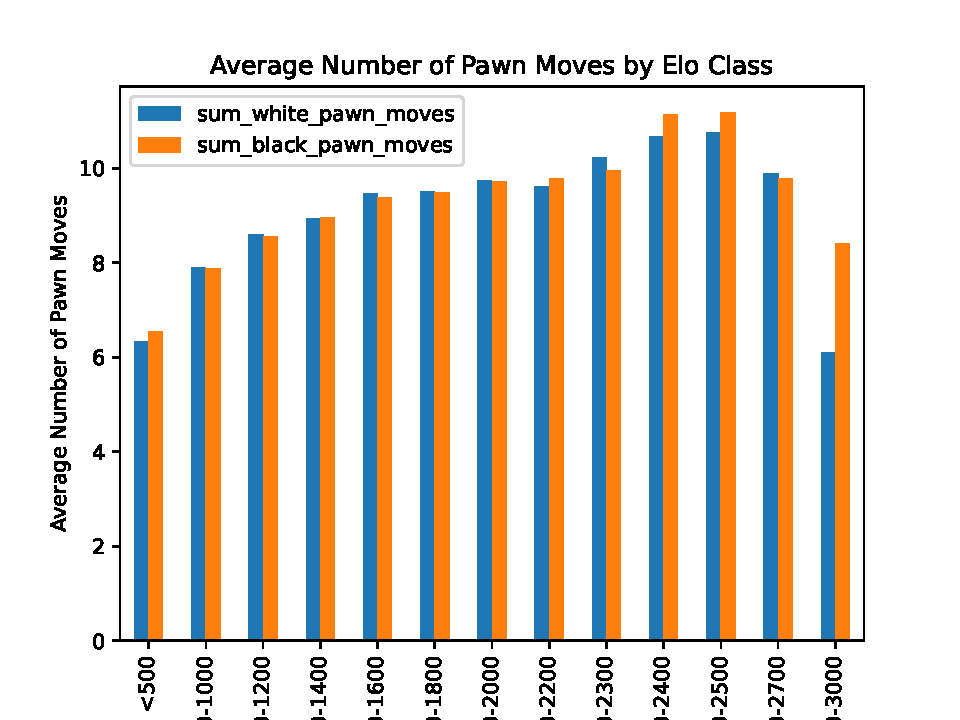
\includegraphics{fig1}
  \caption{}
  \label{}
\end{figure}

\begin{figure}
  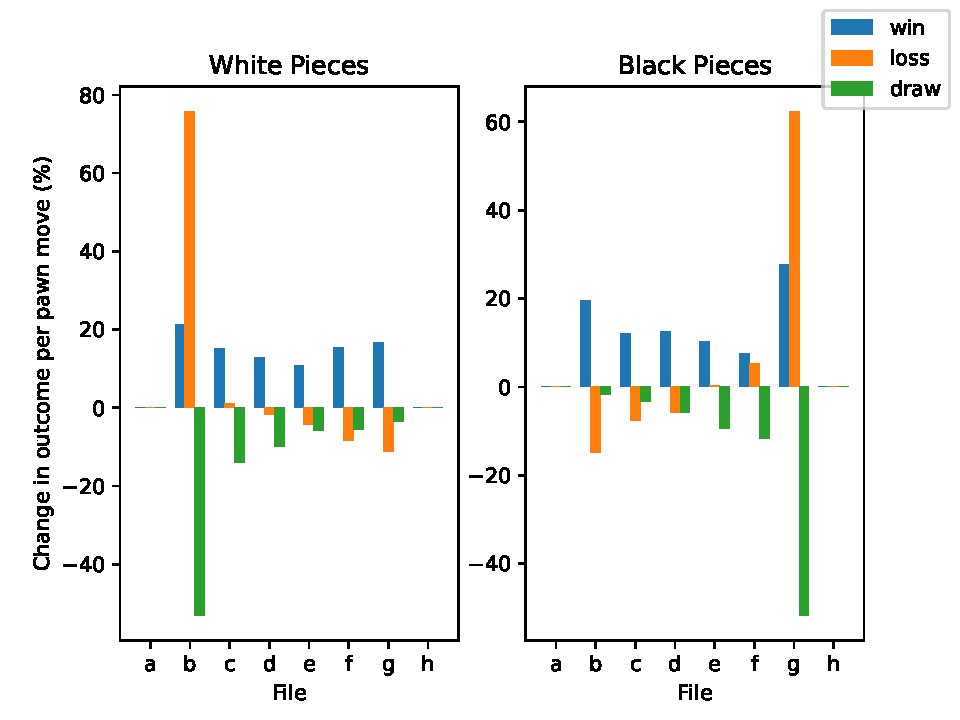
\includegraphics{fig3}
  \caption{Logistic regression results for white and black pieces.}
  \label{}
\end{figure}

\begin{figure}
  \centering
\begin{tabular}{lrr}
  \toprule
  {} &  White Score &  Black Score \\
  \midrule
  Accuracy  &     0.536876 &     0.554375 \\
  Precision &     0.554671 &     0.534788 \\
  Recall    &     0.536876 &     0.554375 \\
  AUC-ROC   &     0.639057 &     0.645282 \\
  \bottomrule
  \end{tabular}
  \caption{}
\end{figure}
\begin{figure}
  \centering
  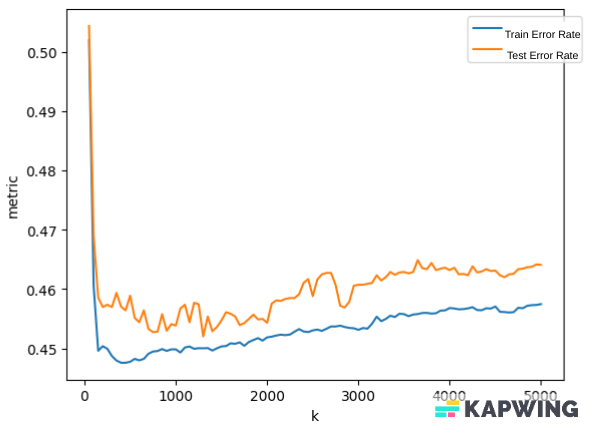
\includegraphics{fig4}
  \caption{}
\end{figure}

% figure 5
\begin{figure}
  \centering
\begin{tabular}{lrr}
  \toprule
  {} &  White Score &  Black Score \\
  \midrule
  Accuracy         &     0.558792 &      0.566343 \\
  Bias             &     0.441870 &      0.441390 \\
  Variance         &     0.212602 &      0.238316 \\
  Train Error Rate &     0.433277 &      0.427884 \\
  Test Error Rate  &     0.441870 &      0.441390 \\
  \bottomrule
  \end{tabular}
  \caption{}
\end{figure}



In chess theory, an understanding of pawns and pawn structure are often highlighted as what differenciates amatures from higher level player CITE, but can such a simple metric as pawn activity show the level of a player. 
  By grouping the games by elo class CITE we can visualise the trend in the total number of pawn moves for white and black (figure 1). 

It would be foolish to assume that there is a linear relationship between the number of pawns pushed and achiving a higher rating, 
instead a two logistic regression model was trained to classify games as a win, loss or draw, from the number of pawn moves made in each file. 
One model was trained for each color due to the slight advantage white obtains from playing first. Both models used a 80/20 train/test data split and have metrics outlined in figure 2. 

Using the regression coeffients, we can plot the percentage change in the liklihood of the result of the game for a one unit increase in the number of pawn moves 
in that rank (figure 3).
Percentage change is calculated as \[p = (e^{c}-1)\cdot 100\] where \(c\) is a coefficient of the regression. 

The low accuracy of the regression model removes some significance from the results, so a 400-Nearest-Neighbours classification was also implemented. 
We used a 60/20/20 split for training, testing and validation sets. 
\(k=400\) was selected as the approprate hyperparameter for the model through testing values of k between 1 and 5000 and comparing train and test error rate (figure 4).   
Metrics were retrieved using a ten fold cross validation which gave a similar accuracy to the previous logistic regression model (figure 5).  


\section{Discussion and conclusions}

% Suggested 400 words.

\paragraph{Summary of findings}
The initial logistic regression model predicts that the most influential file for white is by far the b file, and for black the g file.
In particular, for each pawn move white makes in the b file, this model describes a 22\% increase in the liklihood of the game being classed as a win, 
a 77\% increase in the liklihood of the game being classed as a loss, and a 52\% decrease in the liklihood of the gam being classed as a draw.
Likewise for each pawn move black makes in the g file, the model decribes a 27\% increase in the liklihood of the game being classed as a win, a 61\% increase in 
the liklihood of the game being classed as a loss, and a 49\% decrease in the liklihood of the game being classed as a draw. 

This indicates that controlling the b file is critical for white, and controlling the g file is critical for black, in order to increase the chances of winning. 
This also suggests that playing defensively (i.e. making less pawn moves) may reduce the liklihood of a win due to the correlation of pawn activity here and losing 
or drawing. 
Apart from these files, we can see that pawn activity in the center files (c, d, e, f) increases the likelihood of winning more than any other outcome for both 
colours (excluding black for the f file). This correlates to basic theory on the importance of conrolling the center in chess.lso suggests that playing offensively 
(i.e making more pawn moves) on these files has a greater benifit than playing passively.




\paragraph{Evaluation of own work: strengths and limitations}
Chess is a highly complex game and attempting to predicting the outcom eof a game is an unsolved problem with all the information on a game, nevermind juts the number of pawn moves per file. With this in mind, while the accuracy of model was 20\% above random selection, this value is still far below the standard in most classification models.
The low accuracy can also be attributed to the size of the dataset, which when reduced to only pawn move counts, lacks variance and holds a bias, as demonstated in figure 4. 
The lack of information on the influence of the a and h files can be attributed to these being the only files with only one neighbouring pawn, therefore less pawns capture into this file, reducing the overall number of pawn moves here. 
\paragraph{Comparison with any other related work}
E.g. ``Anscombe has also demonstrated that many patterns of data can
have the same correlation coefficient'' \cite{anscombe1973graphs}.

Wikipedia can also be cited but it is better if you find the original
reference it for a particular claim in the list of references on the
Wikipedia page, read it, and cite it.

The golden rule is always to cite information that has come from other
sources, to avoid plagiarism \cite{wiki:plagarism}.

\paragraph{Improvements and extensions}


\printbibliography
\end{document}

% LocalWords:  lrrrrrrr ment Macduff Kemnay Ruchill FDS mc th fds
% LocalWords:  Anscombe